\chapter{Background}\label{chap:background}

\section{Additive Models with Interactions}

We consider models of the form
\begin{equation}\label{eq:additive-model}
    F(\mathbf{x}) = f_0 + \sum_{i=1}^{d} f_i(x_i) + \sum_{i < j} f_{ij}(x_i, x_j) + \cdots,
\end{equation}
where $f_0 \in \mathbb{R}$ is an intercept, $f_i\colon \mathbb{R} \to \mathbb{R}$ are univariate \emph{main effects}, and $f_{ij}\colon \mathbb{R}^2 \to \mathbb{R}$ are bivariate \emph{interaction effects}.
This class includes \glspl{GAM} \citep{hastie1986generalized}, \glspl{GA2M} \citep{lou2013accurate}, and \glspl{EBM} \citep{nori2019interpretml}.
The appeal is interpretability: each $f_i$ can be plotted as a curve and each $f_{ij}$ as a surface.

\section{The Identifiability Problem}\label{sec:identifiability}

Despite this appeal, the decomposition in \cref{eq:additive-model} is \textbf{not unique}.
For any function $h(x_i)$, one can replace
\[
    f_i(x_i) \leftarrow f_i(x_i) + h(x_i), \qquad f_{ij}(x_i, x_j) \leftarrow f_{ij}(x_i, x_j) - h(x_i),
\]
without changing the overall predictor $F$.
Without additional constraints, the attribution of variance to ``main effects'' versus ``interactions'' is arbitrary.

As a concrete example, consider $F(x_1, x_2) = x_1 \cdot x_2$ on $\{0,1\}^2$.
One parameterization places all variance in the interaction:
\[
    f_0 = 0, \quad f_1 = f_2 = 0, \quad f_{12}(x_1, x_2) = x_1 \cdot x_2.
\]
Another (the fANOVA under uniform weights) shifts mass into the mains:
\[
    f_0 = \tfrac{1}{4}, \quad f_1(x_1) = \tfrac{1}{2}(x_1 - \tfrac{1}{2}), \quad f_2(x_2) = \tfrac{1}{2}(x_2 - \tfrac{1}{2}), \quad f_{12}(x_1, x_2) = (x_1 - \tfrac{1}{2})(x_2 - \tfrac{1}{2}).
\]
Both represent the same function, yet the first attributes all variance to the interaction while the second distributes it equally among $f_1$, $f_2$, and $f_{12}$.

\section{Functional ANOVA Decomposition}\label{sec:fanova}

The \gls{fANOVA} provides a canonical resolution.
Given a weight function $w(\mathbf{x}) \geq 0$ with $\int w(\mathbf{x})\,d\mathbf{x} = 1$, it decomposes $F$ into \textbf{orthogonal} components:
\begin{equation}\label{eq:fanova}
    F(\mathbf{x}) = f_0 + \sum_{u \subseteq \{1,\ldots,d\}} f_u(\mathbf{x}_u),
\end{equation}
subject to the \emph{integrate-to-zero} constraint:
\begin{equation}\label{eq:integrate-to-zero}
    \boxed{\Ew[f_u(\mathbf{x}_u) \mid \mathbf{x}_{u \setminus \{i\}}] = 0 \quad \forall\, i \in u.}
\end{equation}
For a main effect, this requires $\Ew[f_i] = 0$; for an interaction, $\Ew[f_{ij} \mid x_i] = 0$ and $\Ew[f_{ij} \mid x_j] = 0$.
The resulting decomposition is unique and yields orthogonality ($\Ew[f_u \cdot f_v] = 0$ for $u \neq v$) and variance decomposition ($\Varw(F) = \sum_u \Varw(f_u)$) \citep{hooker2007generalized, sobol2001global}.

\section{Piecewise-Constant Case: Tensors and Slice Mean-Zero}\label{sec:tensor-formulation}

For tree ensembles, each feature $x_i$ is discretized into $B_i$ bins.
Main effects become vectors $\mathbf{f}_i \in \mathbb{R}^{B_i}$ and interactions become matrices $\mathbf{F}_{ij} \in \mathbb{R}^{B_i \times B_j}$.
The integrate-to-zero constraint becomes the \emph{weighted slice mean-zero} constraint:
\begin{align}
    \text{Row constraint:} &\quad \sum_{k=1}^{B_j} \mathbf{F}_{ij}[r, k] \cdot w_j[k] = 0 \quad \forall\, r, \label{eq:row-constraint} \\
    \text{Column constraint:} &\quad \sum_{k=1}^{B_i} \mathbf{F}_{ij}[k, c] \cdot w_i[k] = 0 \quad \forall\, c. \label{eq:col-constraint}
\end{align}

\section{Weight Estimation}\label{sec:weights}

The \gls{fANOVA} depends on the weighting distribution $w$, which must be estimated in practice.
\citet{lengerich2020purifying} discuss several estimators:

\begin{description}
    \item[Uniform ($\wunif$):] Equal weight to all bin combinations: $w(\mathbf{x}) \propto 1$.
    \item[Empirical ($\wemp$):] Weights proportional to observed bin counts: $w(\mathbf{x}) \propto \hat{p}(\mathbf{x})$.
    \item[Laplace ($\wlap$):] Smoothed blend $\wlap \propto \wemp + \wunif$, adding pseudo-counts to avoid zero-weight bins.
    \item[Independence-assumed ($\windep$):] Product of marginals: $\windep(\mathbf{x}) = \prod_i \hat{p}(x_i)$.
    \item[Permutation joint ($\wperm$):] Empirical joint on data with columns independently shuffled.
\end{description}

The choice has no effect on predictions but profoundly affects variance attribution, especially when features are dependent.
\Cref{fig:weight-1d} contrasts uniform and empirical marginal weights for a single feature.

\begin{figure}[H]
\centering
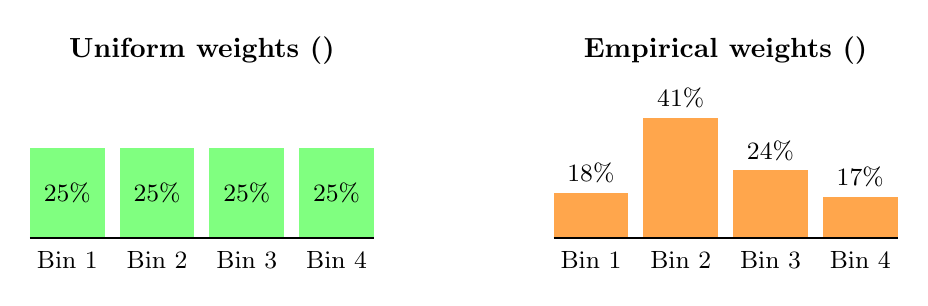
\begin{tikzpicture}[scale=0.95]
  \begin{scope}[xshift=0cm]
    \node[font=\bfseries] at (2.3,2.5) {Uniform weights ($\wunif$)};
    \fill[green!50] (0,0) rectangle (1,1.2);
    \fill[green!50] (1.2,0) rectangle (2.2,1.2);
    \fill[green!50] (2.4,0) rectangle (3.4,1.2);
    \fill[green!50] (3.6,0) rectangle (4.6,1.2);
    \draw[thick] (0,0) -- (4.6,0);
    \node[font=\small] at (0.5,0.6) {25\%};
    \node[font=\small] at (1.7,0.6) {25\%};
    \node[font=\small] at (2.9,0.6) {25\%};
    \node[font=\small] at (4.1,0.6) {25\%};
    \node[font=\small] at (0.5,-0.3) {Bin 1};
    \node[font=\small] at (1.7,-0.3) {Bin 2};
    \node[font=\small] at (2.9,-0.3) {Bin 3};
    \node[font=\small] at (4.1,-0.3) {Bin 4};
  \end{scope}
  \begin{scope}[xshift=7cm]
    \node[font=\bfseries] at (2.3,2.5) {Empirical weights ($\wemp$)};
    \fill[orange!70] (0,0) rectangle (1,0.6);
    \fill[orange!70] (1.2,0) rectangle (2.2,1.6);
    \fill[orange!70] (2.4,0) rectangle (3.4,0.9);
    \fill[orange!70] (3.6,0) rectangle (4.6,0.55);
    \draw[thick] (0,0) -- (4.6,0);
    \node[font=\small,above] at (0.5,0.6) {18\%};
    \node[font=\small,above] at (1.7,1.6) {41\%};
    \node[font=\small,above] at (2.9,0.9) {24\%};
    \node[font=\small,above] at (4.1,0.55) {17\%};
    \node[font=\small] at (0.5,-0.3) {Bin 1};
    \node[font=\small] at (1.7,-0.3) {Bin 2};
    \node[font=\small] at (2.9,-0.3) {Bin 3};
    \node[font=\small] at (4.1,-0.3) {Bin 4};
  \end{scope}
\end{tikzpicture}
\caption[Uniform vs.\ empirical marginal weights.]{Marginal weights for a single feature. Under $\wunif$ (left), all bins are weighted equally. Under $\wemp$ (right), weights reflect the data distribution.}
\label{fig:weight-1d}
\end{figure}

\subsection{Joint Weights and Feature Dependence}\label{sec:joint-weights}

For pairwise interactions, the joint weight matrix $\mathbf{W}_{ij}$ determines the slice mean-zero constraint.
\Cref{fig:weight-2d} compares $\wemp$ with $\windep$ for two correlated features: under $\wemp$, mass concentrates along the diagonal; under $\windep$, it spreads as the product of marginals.
Since purification subtracts weighted slice means, these produce different purified effects.

\begin{figure}[H]
\centering
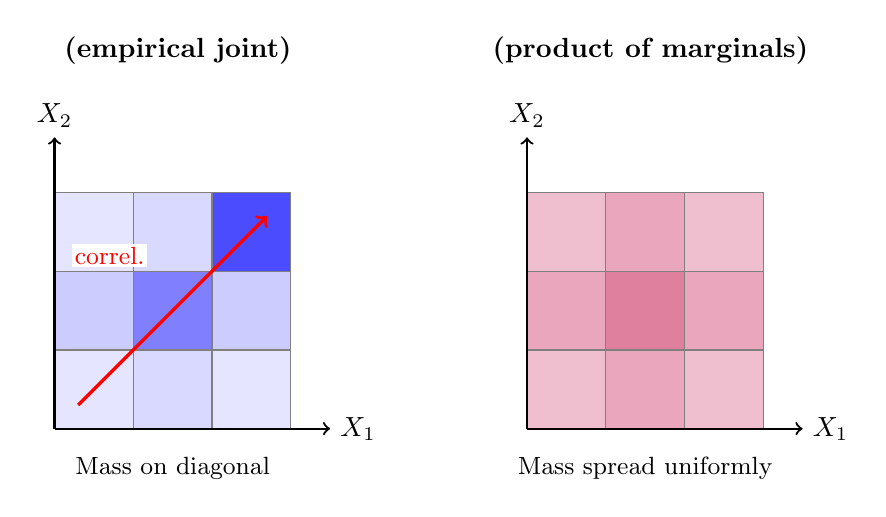
\begin{tikzpicture}[scale=1.0]
  \begin{scope}[xshift=0cm]
    \node[font=\bfseries] at (1.5,4.8) {$\wemp$ (empirical joint)};
    \fill[blue!10] (0,0) rectangle (1,1);
    \fill[blue!50] (1,1) rectangle (2,2);
    \fill[blue!70] (2,2) rectangle (3,3);
    \fill[blue!20] (0,1) rectangle (1,2);
    \fill[blue!15] (1,0) rectangle (2,1);
    \fill[blue!10] (2,0) rectangle (3,1);
    \fill[blue!10] (0,2) rectangle (1,3);
    \fill[blue!15] (1,2) rectangle (2,3);
    \fill[blue!20] (2,1) rectangle (3,2);
    \draw[step=1,gray,thin] (0,0) grid (3,3);
    \draw[->,thick] (0,0) -- (3.5,0) node[right] {$X_1$};
    \draw[->,thick] (0,0) -- (0,3.7) node[above] {$X_2$};
    \draw[->,red,very thick] (0.3,0.3) -- (2.7,2.7);
    \node[red,fill=white,inner sep=1pt,font=\small] at (0.7,2.2) {correl.};
    \node[font=\small] at (1.5,-0.5) {Mass on diagonal};
  \end{scope}
  \begin{scope}[xshift=6cm]
    \node[font=\bfseries] at (1.5,4.8) {$\windep$ (product of marginals)};
    \fill[purple!25] (0,0) rectangle (1,1);
    \fill[purple!35] (1,0) rectangle (2,1);
    \fill[purple!25] (2,0) rectangle (3,1);
    \fill[purple!35] (0,1) rectangle (1,2);
    \fill[purple!50] (1,1) rectangle (2,2);
    \fill[purple!35] (2,1) rectangle (3,2);
    \fill[purple!25] (0,2) rectangle (1,3);
    \fill[purple!35] (1,2) rectangle (2,3);
    \fill[purple!25] (2,2) rectangle (3,3);
    \draw[step=1,gray,thin] (0,0) grid (3,3);
    \draw[->,thick] (0,0) -- (3.5,0) node[right] {$X_1$};
    \draw[->,thick] (0,0) -- (0,3.7) node[above] {$X_2$};
    \node[font=\small] at (1.5,-0.5) {Mass spread uniformly};
  \end{scope}
\end{tikzpicture}
\caption[Empirical joint vs.\ independence-assumed joint weights.]{Joint weight matrices for two correlated features. Under $\wemp$ (left), mass concentrates on the diagonal. Under $\windep$ (right), mass is the product of marginals.}
\label{fig:weight-2d}
\end{figure}
